% MERIT arXiv preprint. PDFLaTeX + standard packages only (arXiv-safe).
% Build locally:  tectonic paper/main.tex   (or pdflatex, twice)
% arXiv tarball:  scripts/make_arxiv_tarball.sh
\documentclass[11pt]{article}

\usepackage[utf8]{inputenc}
\usepackage[T1]{fontenc}
\usepackage[margin=1in]{geometry}
\usepackage{newtxtext,newtxmath}
\usepackage{microtype}
\usepackage{graphicx}
\usepackage{booktabs}
\usepackage{natbib}
\usepackage[hidelinks]{hyperref}
\usepackage{xcolor}

\newcommand{\merit}{\textsc{MERIT}}
\newcommand{\fullrun}[1]{\textcolor{gray}{[\textsc{full run}: #1]}}

\title{When Does Memory Help? A Cost-Aware Evaluation of\\
Long-Term Memory in Tool-Using LLM Agents}
\author{Shweta Mishra\\
Independent Research\\
\texttt{1196shweta@gmail.com}}
\date{July 2026 --- preprint v0.9\thanks{All numbers in \S5 are measured
results from the pilot study (5{,}440 scored episodes, one model). The full
preregistered study (3 models $\times$ 3 seeds $\times$ ${\ge}30$ arcs) is in
progress; this preprint releases the benchmark, harness, and pilot findings.
Passages marked \fullrun{\ldots} will be updated with the larger study.
Code, traces, and preregistration: \url{https://github.com/smshweta/merit-bench}.}}

\begin{document}
\maketitle

\begin{abstract}
Long-term memory is widely assumed to improve the performance of LLM-based
agents, and a rapidly growing ecosystem of memory systems --- retrieval-augmented
stores, rolling summarization, and structured fact memories --- now competes on
conversational recall benchmarks such as LoCoMo and LongMemEval. These
benchmarks measure \emph{question answering over dialogue history}, not the
setting where memory is most consequential in production: \textbf{tool-using
agents executing multi-step tasks across sessions}. We present \merit{}
(Memory Evaluation for Realistic Instrumented Tasks), a benchmark and
evaluation harness that measures the \emph{marginal utility} of memory for
task-executing agents under explicit cost accounting. \merit{} provides
(i)~episodic tool-use tasks in three domains where a controllable fraction of
episodes depend on facts established in earlier episodes, verified
non-re-derivable by an automated leak check; (ii)~a three-tier
\textbf{difficulty ladder} --- single-fact, multi-fact, and \emph{updated-fact}
recall; (iii)~controlled \textbf{memory corruption} (stale, contradiction,
distractor); and (iv)~full token and dollar accounting for every memory
operation. In a pilot study (6 memory conditions $\times$ 3 domains $\times$
3 difficulty tiers, 5{,}440 scored episodes, \texttt{gpt-4.1-mini}), memory
conditions lift dependent-task success from a leak-verified floor of 0.00 (no
memory) to 0.90--1.00 on single-fact tasks (all Holm-adjusted $p \le 0.001$).
The tiers dissociate architectures sharply: when a remembered fact is
\emph{updated} mid-arc, retrieval memory collapses (success 0.20--0.60; it
acts on the correct value only 47\% of the times that value is retrieved),
while a structured fact store with update-on-write semantics stays at
0.90--1.00 --- yet the \emph{hybrid} of the two is worse than the fact store
alone (0.45--0.75). Under explicit cost accounting, the most accurate
condition (full replay) is the least economical: the structured store
delivers equal or better dependent-task success at ${\sim}14\times$ higher
marginal utility per dollar. We release the benchmark, harness, and all
traces for reproducible, cost-aware comparison of agent memory systems.
\end{abstract}

\section{Introduction}

LLM-based agents that plan, call tools, and act over multiple sessions are
moving rapidly into production --- customer support, IT operations, coding, and
personal assistance. A central architectural question for every such
deployment is whether and how to give the agent \emph{long-term memory}:
information persisted across sessions and selectively recalled. A vibrant
ecosystem of memory systems has emerged (Mem0, Letta/MemGPT-style OS
memories, Zep, LangGraph checkpointing, bespoke RAG stores), and vendors
compete on recall benchmarks.

Yet the evaluation of agent memory has three blind spots:

\paragraph{Blind spot 1: Conversational QA is not task execution.}
The dominant benchmarks --- LoCoMo \citep{locomo}, LongMemEval \citep{longmemeval},
and BEAM \citep{beam} --- test whether a system can answer questions about
long, multi-session \emph{conversations}. Production agents, by contrast,
must use remembered facts to \emph{choose the correct tool call}: the right
customer ID, the previously agreed refund amount, the configuration fix
identified during last week's incident. Whether conversational recall scores
transfer to task-execution utility is an open empirical question.

\paragraph{Blind spot 2: Memory is assumed to help; harm is unmeasured.}
Recent work notes that agents sometimes ignore retrieved memory records or
use them inconsistently, and HaluMem \citep{halumem} examines memory
hallucination and consistency --- but in conversational settings. In task
execution, a stale memory (a customer's \emph{old} address, a rolled-back
configuration) is not just unhelpful; it produces a \emph{confidently wrong
action}. No existing benchmark quantifies this failure mode under controlled
corruption, nor the more basic failure our pilot surfaces: agents that
demonstrably hold the correct fact in context and still do not act on it
(Ignore Rate up to 0.53).

\paragraph{Blind spot 3: Cost is reported, but marginal utility is not.}
Memory systems report token counts alongside accuracy, but the decision
practitioners face is economic: does adding memory raise task success enough
to justify its per-task cost? We are not aware of any evaluation that reports
\emph{cost-adjusted marginal utility} --- the change in success probability per
marginal dollar --- across memory architectures.

We address all three with \merit{}. Our contributions:

\begin{enumerate}
\item \textbf{A task suite with controllable memory dependency and
difficulty.} Episodic tool-use tasks in three domains (customer support, IT
operations, personal assistant) where a tunable fraction of episodes depend
on facts established in earlier episodes, and a three-tier difficulty ladder:
\emph{easy} (one fact), \emph{medium} (multiple facts must be composed),
\emph{hard} (the fact is updated mid-arc and the latest value is required).
An automated \textbf{leak check} verifies at generation time that no gold
fact is present in the probe episode's inputs or re-derivable from tools.
\item \textbf{Controlled memory corruption.} Stale, contradictory, and
distractor records injected at known rates $\rho$, with ground-truth flags,
to measure Stale-Memory Harm.
\item \textbf{Three metrics absent from prior evaluations}: Memory
Utilization Rate (MUR), Ignore Rate, and Cost-Adjusted Marginal Utility
(CAMU), computed automatically by the harness (\S\ref{sec:metrics}).
\item \textbf{A pilot study} of 6 memory conditions $\times$ 3 domains
$\times$ 3 difficulty tiers (5{,}440 scored episodes) with preregistered
hypotheses and statistics (paired bootstrap clustered by arc;
Holm--Bonferroni), demonstrating that the benchmark separates memory
architectures that are indistinguishable under single-fact recall.
\fullrun{3 models $\times$ 3 seeds $\times$ ${\ge}30$ arcs}
\item \textbf{Open-source release} of the benchmark, harness, and all
traces, with a deterministic \$0 mock-model mode that validates the full
pipeline.
\end{enumerate}

\section{Related Work}

\subsection{Memory systems for LLM agents}

MemGPT \citep{memgpt} frames memory as an OS-style hierarchy with the LLM
paging information in and out of context. Mem0 \citep{mem0} extracts and
consolidates structured facts at write time; Zep \citep{zep} maintains a
temporal knowledge graph; A-Mem \citep{amem} organizes agentic notes
dynamically. Rolling summarization is the default pattern in agent frameworks
such as LangChain/LangGraph. These systems papers evaluate primarily on
conversational QA (LoCoMo, LongMemEval); none evaluate task-execution utility
under cost accounting. \merit{}'s conditions C1--C5 are deliberately
\emph{reimplementations of these architecture families} under one interface,
so that architectural mechanisms (retrieval, summarization, update-on-write,
hybrid) can be compared in isolation from product engineering.

\subsection{Benchmarks for agent memory}

LoCoMo \citep{locomo} evaluates QA over very long multi-session dialogues.
LongMemEval \citep{longmemeval} covers information extraction, multi-session
reasoning, temporal reasoning, knowledge updates, and abstention over
${\sim}$115K-token histories. BEAM \citep{beam} scales conversational probing
to 10M tokens. HaluMem \citep{halumem} evaluates hallucination at the level
of memory operations (extraction, updating, QA). RealMem \citep{realmem}
moves toward project-oriented interaction. All are \emph{answer-producing}
evaluations; \merit{} is \emph{action-producing}: success is a predicate over
the final state of a mutable world, and the knowledge-update dimension that
LongMemEval and HaluMem probe conversationally becomes, in \merit{}'s hard
tier, a behavioral test of whether the agent \emph{acts} on the latest value.
Long-context benchmarks (RULER, \citealp{ruler}; BABILong, \citealp{babilong})
test single-pass attention over a given context, not the write-and-retrieve
loop of a persistent memory.

\subsection{Tool-use and agent benchmarks}

$\tau$-bench \citep{taubench} evaluates tool-calling agents conversing with
simulated users over domain APIs with database-state success checks --- the
closest environment design to \merit{}'s --- but each task is a single episode;
memory across episodes is not exercised. AgentBench \citep{agentbench},
SWE-bench \citep{swebench}, and WebArena \citep{webarena} similarly evaluate
within-episode competence. \merit{} adds the cross-episode dependency
structure (arcs, plants, probes, leak check) on top of a $\tau$-bench-style
environment.

\subsection{Reliability of agents}

Production reports consistently rank reliability as the top barrier to agent
deployment; confidently-wrong actions are costlier than abstentions.
Stale-memory harm is a concrete, measurable instance: \merit{} injects
staleness at known rates and measures both the success drop and whether the
agent re-verifies before acting.

\section{The \merit{} Benchmark}

\subsection{Design goals}

G1 (Ecological validity): tasks require tool calls with programmatically
verifiable end states. G2 (Controllable dependency and difficulty): the
dependent-task ratio and the difficulty tier are benchmark parameters. G3
(Adversarial realism): corruption reflects real staleness processes. G4 (Cost
transparency): every token in and out of the memory system is metered. G5
(Reproducibility): deterministic seeded worlds, scripted or cached simulated
users, pinned model versions, released traces, and a \$0 deterministic mock
model that exercises the entire pipeline.

\subsection{Environment}

An \textbf{episode} is one agent session with a simulated user and a tool API
over a mutable world state (SQLite). Episodes are grouped into \textbf{arcs}
of 4--6 episodes sharing entities. Arcs contain \textbf{plant} episodes (a
fact is established conversationally; the user explicitly forbids acting on
it yet), optional \textbf{update} episodes (the fact is revised),
\textbf{probe} episodes (success requires the fact; it is absent from the
episode's inputs), and \textbf{independent} episodes (solvable
within-episode).

Two safeguards proved essential in practice. The \textbf{leak check} asserts
at generation time that every gold fact value is absent from the probe
episode's inputs and from the initial world state, with gold values kept
unique arc-wide. \textbf{Delta scoring} marks an episode successful only if
its checker predicate flips from false to true \emph{during} that episode ---
in early gate runs, eager agents processed refunds during plant episodes, and
probes then ``succeeded'' off inherited world state; delta scoring eliminates
this world-state leak channel entirely (0 contaminated episodes in 5{,}440).

\subsection{Domains}

\begin{itemize}
\item \textbf{D1 Customer support (retail):} tools = \texttt{get\_order},
\texttt{refund}, \texttt{update\_address}, \texttt{get\_policy},
\texttt{send\_message}. Facts: agreed partial-refund amounts, updated
addresses.
\item \textbf{D2 IT operations:} tools = \texttt{search\_logs},
\texttt{get\_deploy\_history}, \texttt{get\_config}, \texttt{set\_config},
\texttt{deploy}, \texttt{update\_ticket}. Facts: diagnosed config fixes, safe
rollback versions.
\item \textbf{D3 Personal assistant:} tools = \texttt{get\_calendar},
\texttt{create\_event}, \texttt{send\_email}, \texttt{get\_preference},
\texttt{set\_preference}. Facts: standing room/time preferences, dinner
commitments (place, day, time).
\end{itemize}

\subsection{Difficulty ladder and memory conditions}

\textbf{Difficulty}: \emph{easy} = one gold fact per probe; \emph{medium} =
multi-fact probes (every gold value must appear in the executed tool calls);
\emph{hard} = updated-fact probes: the value is planted, revised in a later
episode, and the probe requires the \textbf{latest} value. The hard tier is a
targeted stressor for the architectural distinction between stores that
overwrite (update-on-write) and stores that accumulate (replay, retrieval).

\textbf{Memory conditions}, one interface (\texttt{write(episode)},
\texttt{read(context)}): C0 none; C1 full replay of prior transcripts; C2
retrieval (pilot: keyword-overlap retrieval; \fullrun{embedding retrieval});
C3 rolling summary (pilot: extractive truncation; \fullrun{LLM
summarization}); C4 structured fact store with update-on-write (pilot:
pattern-based extraction; \fullrun{LLM extraction}); C5 hybrid (C4 + C2). All
conditions share the same agent scaffold (ReAct-style tool loop;
\citealp{react}), prompts (except the memory block), tools, and decoding
(temperature 0).

\subsection{Metrics}\label{sec:metrics}

\begin{itemize}
\item \textbf{TSR}: task success rate by programmatic end-state check, split
by dependent/independent.
\item \textbf{MUR}: among dependent episodes where all gold values were
present in the retrieved memory block, the fraction where every gold value
appears in the executed tool-call arguments (value tracing). \fullrun{validated
by a 100-episode human audit with a second annotator; Cohen's $\kappa$}
\item \textbf{Ignore Rate} $= 1 - \mathrm{MUR}$ on episodes with correct
memory present.
\item \textbf{SMH}: $\mathrm{TSR}(\text{clean}) -
\mathrm{TSR}(\text{corrupted})$ at $\rho \in \{0.1, 0.3\}$ for stale /
contradiction / distractor corruption.
\item \textbf{Cost \& CAMU}: metered tokens and dollars per episode;
$\mathrm{CAMU} = \Delta\mathrm{TSR}$ vs.\ C0 per $\Delta$cost vs.\ C0;
break-even task value $= \Delta\text{cost}/\Delta\mathrm{TSR}$.
\end{itemize}

\subsection{Statistical methodology}

Paired comparisons on identical task instances; 95\% CIs and two-sided $p$ by
paired bootstrap (10{,}000 resamples) clustered at the arc level;
Holm--Bonferroni within each preregistered hypothesis family (H1--H4,
committed to the public repository before experiments; commit history is the
preregistration record).

\section{Experimental Setup (Pilot)}

Model: \texttt{gpt-4.1-mini} (pinned; temperature 0). Scale: 10 arcs
$\times$ 5 episodes per (domain $\times$ difficulty $\times$ condition);
dependent-task ratio 0.5; corruption sweep (3 modes $\times$ $\rho \in \{0.1,
0.3\}$) and LLM-paraphrased users on D1. Totals: \textbf{5{,}440 scored
episodes, \$4.61 in API cost} (${\sim}\$0.0008$/episode). Harness: Python,
LiteLLM for provider-agnostic calls and metering; SQLite worlds; scripted
simulated users (LLM paraphrase mode with a paraphrase-leak check on D1). The
mock-model mode replays the entire grid deterministically at \$0 and is
exercised by 62 unit tests, including generation determinism, leak checks,
and end-to-end pipeline invariants. \fullrun{+ frontier API model +
open-weight model via vLLM, 3 seeds, ${\ge}30$ arcs, corruption + LLM users
on all domains}

\section{Results (Pilot)}

\subsection{Memory helps on dependent tasks; the floor is real}

C0 scored \textbf{0.000} on dependent tasks in all nine (domain $\times$
difficulty) cells --- the leak check holds; there is no route to the gold facts
except memory. On independent tasks C0 scores 0.88--1.00, confirming task
solvability. Every memory condition beats C0 on dependent tasks in every
domain at easy difficulty ($\Delta$TSR $+0.55$ to $+1.00$; all Holm-adjusted
$p \le 0.001$, paired bootstrap clustered by arc).

\subsection{The difficulty ladder dissociates architectures}\label{sec:ladder}

\begin{table}[t]
\centering
\caption{Dependent-task TSR by difficulty tier and memory condition
(D1~/~D2~/~D3). See also Figure~\ref{fig:ladder}.}
\label{tab:ladder}
\small
\begin{tabular}{lccccc}
\toprule
Tier & C1 replay & C2 retrieval & C3 summary & C4 facts & C5 hybrid \\
\midrule
easy   & 1.00 / 1.00 / 0.90 & 0.95 / 1.00 / 0.95 & 0.55 / 0.65 / 0.40 & 1.00 / 0.60 / 0.90 & 0.95 / 1.00 / 1.00 \\
medium & 0.55 / 1.00 / 0.90 & 0.30 / 0.85 / 0.90 & 0.30 / 0.40 / 0.50 & 0.85 / 1.00 / 0.80 & 0.85 / 1.00 / 1.00 \\
hard   & 1.00 / 1.00 / 1.00 & 0.60 / 0.25 / 0.20 & 0.00 / 0.15 / 0.00 & 1.00 / 0.90 / 1.00 & 0.70 / 0.45 / 0.75 \\
\bottomrule
\end{tabular}
\end{table}

\begin{figure}[t]
\centering
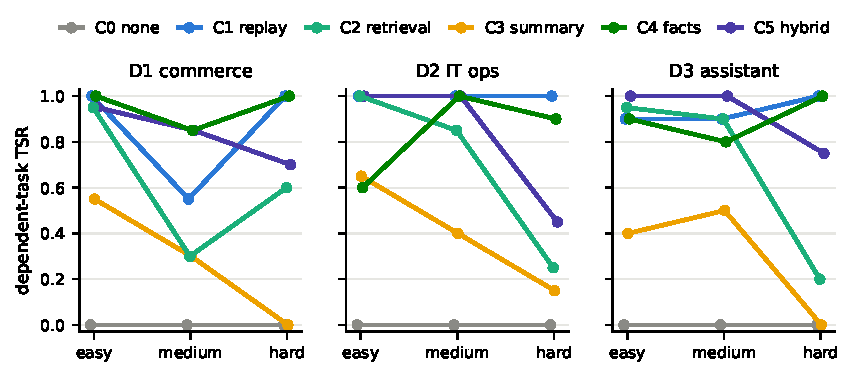
\includegraphics[width=\textwidth]{figures/fig1_difficulty_ladder.pdf}
\caption{Dependent-task TSR across the difficulty ladder, per memory
condition and domain. The hard (updated-fact) tier separates stores that
overwrite (C4) or replay chronology (C1) from retrieval-based stores (C2, C5)
and lossy summaries (C3).}
\label{fig:ladder}
\end{figure}

Table~\ref{tab:ladder} and Figure~\ref{fig:ladder} show three dissociations:
(1)~\textbf{Updated facts break retrieval memory}: C2 falls to 0.20--0.60 on
hard while C4 stays at 0.90--1.00 --- retrieval surfaces stale and fresh values
side by side with no recency signal, while update-on-write overwrites.
(2)~\textbf{Hybrid is worse than its better half} on hard (0.45--0.75 vs.\
C4's 0.90--1.00): the retrieval half re-imports the staleness the fact store
had eliminated. (3)~\textbf{Full replay is update-immune but
composition-limited}: C1 resolves recency from chronology (1.00 on hard) yet
drops to 0.55 on D1-medium despite containing every fact --- possessing
information and composing it are different capabilities.

\subsection{Agents ignore memories they hold}

On the hard tier, pooling domains, the correct (latest) value was present in
C2's retrieved block in 45 probe episodes; the agent acted on it in 21
(\textbf{Ignore Rate 0.53}). Even C1/C4, whose memory blocks are clean, show
Ignore Rates up to 0.45 in multi-fact (medium-tier) episodes
(Figure~\ref{fig:ignore}). This is Blind spot~2 made measurable:
memory-system accuracy overstates end-task benefit unless utilization is
measured.

\begin{figure}[t]
\centering
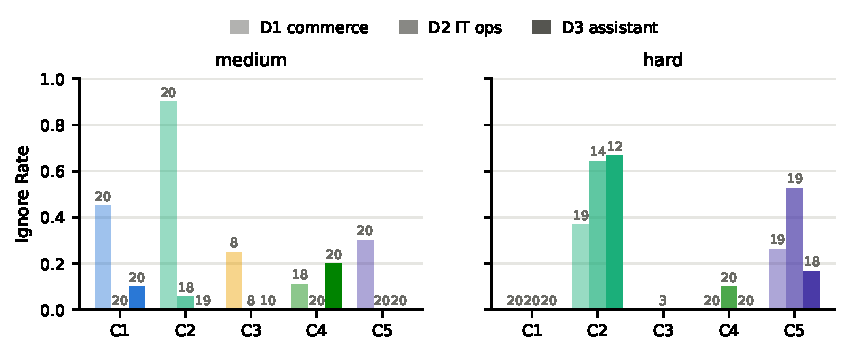
\includegraphics[width=\textwidth]{figures/fig2_ignore_rate.pdf}
\caption{Ignore Rate --- the fraction of dependent episodes where every gold
value was present in the memory block but the agent did not act on it --- by
condition and domain on the medium and hard tiers. Numbers above bars are
episode counts with memory present (bars at zero are shown by their count
only).}
\label{fig:ignore}
\end{figure}

\subsection{Stale-memory harm}

On D1 with stale corruption at $\rho = 0.3$ (Figure~\ref{fig:smh}), TSR on
dependent tasks drops by 0.05--0.25 depending on condition; the largest and
only Holm-significant harms in the pilot are on the hybrid C5 (SMH $+0.20$ at
$\rho = 0.1$, $+0.25$ at $\rho = 0.3$), while C4 shows the smallest harm
(${\le}0.05$) --- consistent with update-on-write limiting the blast radius of
stale records. Contradiction and distractor corruption produce smaller,
mostly non-significant harms at pilot scale. \fullrun{corruption sweeps on
all domains with verification-rate analysis}

\begin{figure}[t]
\centering
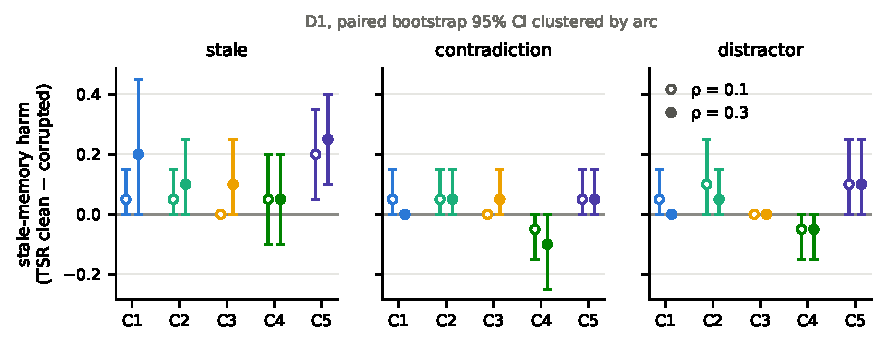
\includegraphics[width=\textwidth]{figures/fig3_stale_memory_harm.pdf}
\caption{Stale-memory harm (TSR clean $-$ corrupted, dependent tasks, D1) by
condition, corruption mode, and corruption rate $\rho$; error bars are paired
bootstrap 95\% CIs clustered by arc.}
\label{fig:smh}
\end{figure}

\subsection{Cost and marginal utility}

Per-episode cost on D1-easy (Figure~\ref{fig:cost}): C0 \$0.00046, C4
\$0.00052, C5 \$0.00076, C2 \$0.00078, C3 \$0.00088, C1 \$0.00129 (2{,}986
tokens/episode --- $3.4\times$ C0). CAMU ranking inverts the accuracy ranking
(H4 supported in all three domains): C4 delivers ${\sim}17{,}300$ percentage
points of dependent-task success per marginal dollar on D1 vs.\
${\sim}1{,}200$ for C1; in D2, C4's marginal cost was \emph{negative}
(compact fact notes shrank prompts below the no-memory baseline) while adding
$+60$ points. Break-even task values at pilot prices are fractions of a cent
per task for all conditions --- memory pays for itself at trivially low task
values \emph{when it works}; the practitioner-relevant differences are in
robustness (\S\ref{sec:ladder}--5.4), not raw affordability, at these model
prices.

\begin{figure}[t]
\centering
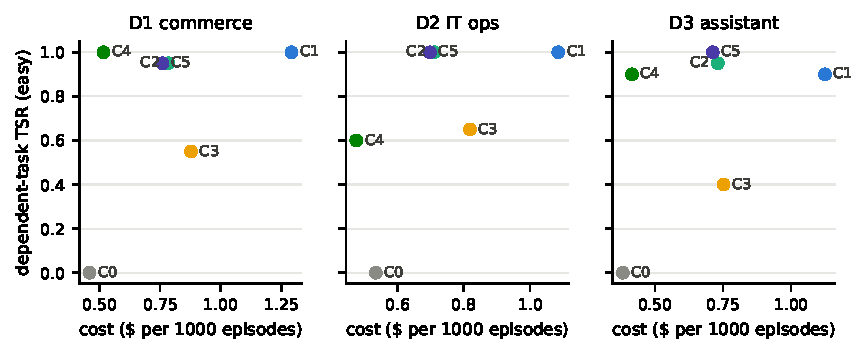
\includegraphics[width=\textwidth]{figures/fig4_cost_frontier.pdf}
\caption{Metered cost per episode vs.\ dependent-task TSR at the easy tier.
C4 sits at or near the Pareto frontier in all domains; in D2 and D3 its
compact fact notes make it cheaper than several alternatives while C1 full
replay pays a 2--3$\times$ token premium for the same or lower TSR.}
\label{fig:cost}
\end{figure}

\subsection{What the pilot cannot yet say}

Single model, single seed, 10 arcs per cell, and starter implementations of
C2/C3/C4 (keyword retrieval, truncation summaries, pattern extraction). The
C3 results in particular are a floor, not an estimate, for LLM-summarization
memory; C4's pattern extractor required domain-specific patterns (an
instructive brittleness --- see \S\ref{sec:discussion}). The full run upgrades
all three and adds models/seeds/arcs. We report the pilot because the
\emph{dissociations} in \S\ref{sec:ladder} are architectural in origin and
large (0.4--0.8 absolute TSR), and because the benchmark itself --- not the
leaderboard --- is the contribution.

\section{Discussion}\label{sec:discussion}

\paragraph{Practitioner guidance (provisional).}
If tasks depend on facts that get \emph{revised} (addresses, configs,
schedules --- most operational facts), prefer update-on-write structured memory
over retrieval; do not assume a hybrid inherits the better component's
behavior --- measure it. Full replay is a strong accuracy baseline that fails
on cost ($3.4\times$ tokens) and on multi-fact composition. Rolling summaries
need real summarization; truncation is not a memory system.

\paragraph{Why do agents ignore correct memories?}
Traces show two patterns: (i)~under retrieval, stale and fresh values
co-occur and the agent averages, asks, or picks the stale one (no
provenance/timestamps to arbitrate); (ii)~under multi-fact composition,
agents act on the subset of facts nearest the task phrasing. Both suggest
memory \emph{presentation} (provenance, recency marking, contradiction
surfacing) matters as much as memory \emph{storage}.

\paragraph{Extraction brittleness as a hidden cost.}
C4's economics are the best in every domain, but its pattern-based extractor
was blind outside its home domain until domain patterns were added --- in
production, extraction quality is the tax that structured memory pays. The
full run's LLM extractor moves this cost into the metered CAMU, where it
belongs.

\paragraph{A methodological note.}
Two of our safeguards were added because early runs failed without them:
eager agents leaked gold facts into world state (fixed by delta scoring), and
gold-value collisions leaked across task pairs (fixed by arc-wide
uniqueness). Task-execution memory benchmarks have leak channels that
conversational QA benchmarks cannot express; we recommend leak checks over
\emph{world state}, not just prompts, as standard practice.

\section{Threats to Validity}

\textbf{Construct:} programmatic checkers may not capture all real-world
success notions; the MUR tracer is string containment pending the human
audit. \textbf{Internal:} prompt differences across conditions are confined
to the memory block; delta scoring removes world-state carryover; the
mock-model grid guards the pipeline, but mock results are never reported as
findings. \textbf{External:} one model at pilot scale --- architectural
dissociations may shift with model strength (the full run tests whether
stronger models need memory less or exploit it better); three domains;
synthetic worlds with scripted users (LLM-paraphrase mode mitigates phrasing
overfit on D1). \textbf{Reproducibility:} deterministic seeded generation,
pinned model IDs, released traces, \$0 mock mode; API model drift is
mitigated by the open-weight model in the full run.

\section{Conclusion}

\merit{} reframes agent-memory evaluation from ``can the system recall?'' to
``does recall change what the agent does, at what cost, and how does it
fail?''. Even at pilot scale the answer is not monotone: architectures
indistinguishable on single-fact recall separate by 0.4--0.8 TSR when facts
must be composed or superseded, agents ignore up to half of correctly
retrieved facts, and the most accurate memory is $14\times$ less economical
than the most efficient one. The benchmark, harness, traces, and
preregistration are public; we invite memory-system authors to evaluate
against \merit{}.

\begin{thebibliography}{99}

\bibitem[Bian et al.(2026)]{realmem}
Bian, H., Yao, Z., Hu, S., Xu, Z., Zhang, S., Guo, Y., Yang, Z., Han, X.,
Wang, H., Chen, R. (2026). RealMem: Benchmarking LLMs in Real-World
Memory-Driven Interaction. arXiv:2601.06966.

\bibitem[Chhikara et al.(2025)]{mem0}
Chhikara, P., Khant, D., Aryan, S., Singh, T., Yadav, D. (2025). Mem0:
Building Production-Ready AI Agents with Scalable Long-Term Memory.
arXiv:2504.19413.

\bibitem[Hsieh et al.(2024)]{ruler}
Hsieh, C.-P., et al. (2024). RULER: What's the Real Context Size of Your
Long-Context Language Models? arXiv:2404.06654.

\bibitem[HaluMem(2025)]{halumem}
HaluMem (2025). HaluMem: Evaluating Hallucinations in Memory Systems of
Agents. arXiv:2511.03506.

\bibitem[Jimenez et al.(2024)]{swebench}
Jimenez, C., et al. (2024). SWE-bench: Can Language Models Resolve
Real-World GitHub Issues? ICLR 2024. arXiv:2310.06770.

\bibitem[Kuratov et al.(2024)]{babilong}
Kuratov, Y., et al. (2024). BABILong: Testing the Limits of LLMs with Long
Context Reasoning-in-a-Haystack. arXiv:2402.10790.

\bibitem[Liu et al.(2023)]{agentbench}
Liu, X., et al. (2023). AgentBench: Evaluating LLMs as Agents.
arXiv:2308.03688.

\bibitem[Maharana et al.(2024)]{locomo}
Maharana, A., et al. (2024). Evaluating Very Long-Term Conversational Memory
of LLM Agents (LoCoMo). ACL 2024. arXiv:2402.17753.

\bibitem[Packer et al.(2023)]{memgpt}
Packer, C., et al. (2023). MemGPT: Towards LLMs as Operating Systems.
arXiv:2310.08560.

\bibitem[Rasmussen et al.(2025)]{zep}
Rasmussen, P., et al. (2025). Zep: A Temporal Knowledge Graph Architecture
for Agent Memory. arXiv:2501.13956.

\bibitem[Tavakoli et al.(2026)]{beam}
Tavakoli, M., Salemi, A., Ye, C., Abdalla, M., Zamani, H., Mitchell, J.R.
(2026). Beyond a Million Tokens: Benchmarking and Enhancing Long-Term Memory
in LLMs (BEAM). ICLR 2026. arXiv:2510.27246.

\bibitem[Wu et al.(2025)]{longmemeval}
Wu, D., et al. (2025). LongMemEval: Benchmarking Chat Assistants on
Long-Term Interactive Memory. ICLR 2025. arXiv:2410.10813.

\bibitem[Xu et al.(2025)]{amem}
Xu, W., et al. (2025). A-Mem: Agentic Memory for LLM Agents.
arXiv:2502.12110.

\bibitem[Yao et al.(2024)]{taubench}
Yao, S., Shinn, N., Razavi, P., Narasimhan, K. (2024). $\tau$-bench: A
Benchmark for Tool-Agent-User Interaction in Real-World Domains.
arXiv:2406.12045.

\bibitem[Yao et al.(2023)]{react}
Yao, S., et al. (2023). ReAct: Synergizing Reasoning and Acting in Language
Models. ICLR 2023. arXiv:2210.03629.

\bibitem[Zhou et al.(2023)]{webarena}
Zhou, S., et al. (2023). WebArena: A Realistic Web Environment for Building
Autonomous Agents. arXiv:2307.13854.

\end{thebibliography}

\end{document}
